% Title: gl2ps_renderer figure
% Creator: GL2PS 1.4.0, (C) 1999-2017 C. Geuzaine
% For: Octave
% CreationDate: Thu Nov 28 11:09:18 2019
\setlength{\unitlength}{1pt}
\begin{picture}(0,0)
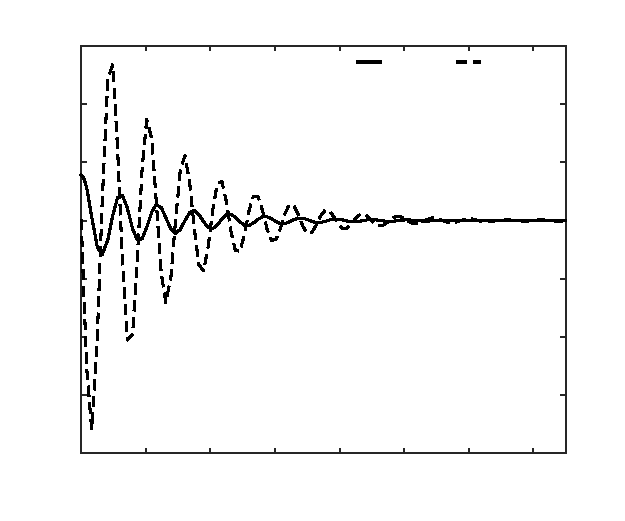
\includegraphics{../Report/img/PosVelF-inc}
\end{picture}%
\begin{picture}(300,250)(0,0)
\fontsize{10}{0}
\selectfont\put(39,25){\makebox(0,0)[t]{\textcolor[rgb]{0.15,0.15,0.15}{{0}}}}
\fontsize{10}{0}
\selectfont\put(70,25){\makebox(0,0)[t]{\textcolor[rgb]{0.15,0.15,0.15}{{2}}}}
\fontsize{10}{0}
\selectfont\put(101,25){\makebox(0,0)[t]{\textcolor[rgb]{0.15,0.15,0.15}{{4}}}}
\fontsize{10}{0}
\selectfont\put(132,25){\makebox(0,0)[t]{\textcolor[rgb]{0.15,0.15,0.15}{{6}}}}
\fontsize{10}{0}
\selectfont\put(163,25){\makebox(0,0)[t]{\textcolor[rgb]{0.15,0.15,0.15}{{8}}}}
\fontsize{10}{0}
\selectfont\put(194,25){\makebox(0,0)[t]{\textcolor[rgb]{0.15,0.15,0.15}{{10}}}}
\fontsize{10}{0}
\selectfont\put(225,25){\makebox(0,0)[t]{\textcolor[rgb]{0.15,0.15,0.15}{{12}}}}
\fontsize{10}{0}
\selectfont\put(256,25){\makebox(0,0)[t]{\textcolor[rgb]{0.15,0.15,0.15}{{14}}}}
\fontsize{10}{0}
\selectfont\put(34.0107,48.7747){\makebox(0,0)[r]{\textcolor[rgb]{0.15,0.15,0.15}{{-10}}}}
\fontsize{10}{0}
\selectfont\put(34.0107,89.5078){\makebox(0,0)[r]{\textcolor[rgb]{0.15,0.15,0.15}{{-5}}}}
\fontsize{10}{0}
\selectfont\put(34.0107,130.241){\makebox(0,0)[r]{\textcolor[rgb]{0.15,0.15,0.15}{{0}}}}
\fontsize{10}{0}
\selectfont\put(34.0107,170.974){\makebox(0,0)[r]{\textcolor[rgb]{0.15,0.15,0.15}{{5}}}}
\fontsize{10}{0}
\selectfont\put(34.0107,211.707){\makebox(0,0)[r]{\textcolor[rgb]{0.15,0.15,0.15}{{10}}}}
\fontsize{11}{0}
\selectfont\put(155.25,12){\makebox(0,0)[t]{\textcolor[rgb]{0.15,0.15,0.15}{{Tiempo}}}}
\fontsize{11}{0}
\selectfont\put(14.0107,130.241){\rotatebox{90}{\makebox(0,0)[b]{\textcolor[rgb]{0.15,0.15,0.15}{{$\theta, \dot{\theta}$}}}}}
\fontsize{11}{0}
\selectfont\put(155.25,238){\makebox(0,0)[b]{\textcolor[rgb]{0,0,0}{{Posición y Velocidad del péndulo}}}}
\fontsize{9}{0}
\selectfont\put(184.094,220.329){\makebox(0,0)[l]{\textcolor[rgb]{0,0,0}{{  $\theta$}}}}
\fontsize{9}{0}
\selectfont\put(231.968,220.329){\makebox(0,0)[l]{\textcolor[rgb]{0,0,0}{{  $\dot{\theta}$}}}}
\end{picture}
